
%!TEX encoding = UTF-8 Unicode
\documentclass[12pt]{scrartcl}
%\usepackage[applemac]{inputenc} % Mac-Umlaute direkt verwenden öäüß
%\usepackage[isolatin]{inputenc} % PC-Umlaute direkt verwenden 
\usepackage[utf8]{inputenc} % Unicode funktioniert unter Windows, Linux und Mac
\usepackage[T1]{fontenc}
\usepackage{times}
\usepackage[ngerman]{babel}
\usepackage{csquotes}
\usepackage[
backend=biber,
bibstyle=ieee,
citestyle=ieee
]{biblatex}
%\usepackage{ngerman}
\usepackage{graphicx}
\usepackage[hidelinks]{hyperref}\urlstyle{rm}
\usepackage{times}
\usepackage[scaled]{helvet}
\usepackage{a4wide}
\usepackage{rotating}
\usepackage{listings}\lstset{breaklines=true,breakatwhitespace=true,frame=leftline,captionpos=b,xleftmargin=6ex,tabsize=4,numbers=left,numberstyle=\ttfamily\footnotesize,basicstyle=\ttfamily\footnotesize}
\sloppy
\setlength{\parindent}{0em}
\setlength{\parskip}{1.2ex plus 0.5ex minus 0.5ex}
\pagestyle{plain}
\addbibresource{sem.bib}

\begin{document}

\newpage
\thispagestyle{empty}
\begin{center}\Large
Universität Hamburg \par
Fachbereich Informatik
\vfill
Seminararbeit
\vfill
{\Large\textsf{\textbf{Vergleich von IPSec und OpenVPN}}\par}
\vfill
vorgelegt von 
\par\bigskip
Mustafa Eris, Jim Martens, Benjamin Scholz \par
%Matrikelnummern 6420323 \par
Studiengang BSc. Informatik
\end{center}

\newpage
\section*{Zusammenfassung}


\newpage
\tableofcontents

\newpage
\section{Vorbemerkung}
Problem: VPN (Virtual Private Network) aufsetzen
Relevanz: sichere Kommunikation zwischen zwei privaten Netzwerken

\section{Grundlagen}
Was sind VPNs? Warum braucht man sie? Wozu werden sie verwendet?
Was ist das OSI-Referenzmodell? Wie ist es aufgebaut?
\section{IPSec}
\subsection{Entstehungsgeschichte}
IPSec ist unter der Aufsicht eines Komitees entstanden. Diese Vorgehensweise wurde dabei gezwungenermaßen auferlegt und erschwerte nach Ansicht vieler Mitwirkender die Arbeit erheblich. \footnote{Ferguson, Niels, and Bruce Schneier. ``A cryptographic evaluation of IPsec.'' Counterpane Internet Security, Inc 3031 (2000).} 
Die Entstehungsweise führte dazu, dass IPSec unnötig kompliziert wurde. Die einen Mitglieder wollten die eine Lösung implementieren und andere plädierten für eine andere Lösung, was dazu führte, dass beide Lösungen implementiert wurden. Dies geht jedoch zu Lasten der Nutzbarkeit. Zu viele Optionen führen nicht nur zur Verwirrung und Komplizierung der Implementation von IPSec bei den Nutzern, es kann vor Allem auch zu Sicherheitslücken führen. Experten bemängelten diese Komplexität.\\
Die erste Version von IPSec ist 1995 spezifiziert worden. Doch über die Jahre ist der Standard immer weiter entwickelt worden und so gibt es eine zweite Version aus 1998 und eine dritte aus 2005. Diese gelten als zwar allgemein als V2 und V3, jedoch sind verschiedene Aspekte von IPSec in verschiedenen sogenannten ``Request for Comments'', kurz RFC, spezifiziert. So gibt es beispielsweise ein RFC, dass sich allgemein auf IPSec bezieht, aktuell RFC 4301 aus 2005, und es gibt beispielsweise ein RFC, dass sich auf die zu verwendenden Verschlüsselungsalgorithmen bezieht, aktuell RFC 7321 bereits aus 2014. So ist gewährleistet, dass IPSec weiterhin auf dem neuesten Stand gehalten werden kann, ohne dass man jedes mal die komplette Spezifikation überarbeiten muss.
Die folgenden RFCs sind für IPSec relevant:
\begin{itemize}
\item RFC 4301: Beschreibt den grundsätzlichen Aufbau von IPSec
\item RFC 4302: Beschreibt den Authentication Header (AH)
\item RFC 4303: Beschreibt Encapsulating Security Payload (ESP)
\item RFC 7321: Gibt vor welche Algorithmen für AH und ESP verwendet werden sollten
\item RFC 5996: Beschreibt das Internet Key Exchange Protocol Version 2 (IKEv2)
\item RFC 4307: Gibt vor welche Algorithmen für IKEv2 verwendet werden sollten
\item RFC 4308: Gibt Empfehlungen für Sammlungen von Algorithmen, die verwendet werden können
\end{itemize}
Es gibt noch viel mehr RFCs die man IPSec zuordnen kann, doch dies sind die wichtigsten. Im folgenden Kapitel werden wir näher auf die technischen Aspekte von IPSec eingehen und die Themen der einzelnen RFCs näher betrachten.

\subsection{Technischer Aufbau}
\subsubsection{Tunnel Modus und Transport Modus}
IPSec kann in zwei verschiedenen Modi betrieben werden: Transport Modus oder Tunnel Modus. 
Beim Tunnel Modus werden die IP-Pakete in neue Pakete verpackt mit einem neuen Header. Dabei werden die Pakete jedoch von den einzelnen Gateways bearbeitet. Das heißt im Endeffekt, dass die Sicherheit nur von Gateway zu Gateway gewährleistet wird und nicht vom einem Ende zum anderen. Der Vorteil ist, dass der Endnutzer die Anwendung nicht merkt, da zum Beispiel der Router dies übernehmen kann. 
Im Transport Modus ist die Sicherheit vom einen zum anderen Ende gewährleistet. Dabei werden die eigentlichen IP-Pakete beibehalten und einige sicherheitsrelevante Felder hinzugefügt.
\subsubsection{Authentication Header}
Der Authentication Header, kurz AH, kann dazu verwendet werden, um die Authentizität und Integrität von Daten zu gewährleisten, und außerdem um Replay-Angriffe abzuwehren. Er muss im Gegensatz zur Alternative `` Encapsulating Security Payload'' jedoch nicht von IPSec Implementationen unterstützt werden.\footnote{RFC 4301 3.2.  How IPsec Works} Der Authentication Header wird dabei an die IP-Pakete angehängt und sieht wie folgt aus:

\begin{figure}[htbp] 
  \centering
     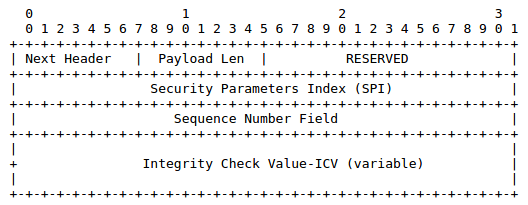
\includegraphics[width=0.7\textwidth]{AH-Aufbau.png}
  \caption{Aufbau des Authentication Headers aus RFC 4302}
  \label{AH-Aufbau}
\end{figure}

Das 8 Bit lange Feld ``Next Header'' gibt an welche Art Nutzdaten nach dem AH folgen. Eine 4 bedeutet zum Beispiel IPv4 und eine 41 IPv6. \\
Das 8 Bit lange Feld ``Payload Length'' gibt die Länge des AH in 4 Byte Worten - 2 an. \\
Das 16 Bit lange Feld ``Reserved'' ist reserviert, damit man es in Zukunft nutzen kann, falls es benötigt wird.\\
Das 32 Bit lange Feld ``Security Parameters Index'' (SPI) enthält die verwendete Security Association, die beim Versenden des Paketes verwendet wurde. Die Security Association beschreibt dabei, welche Sicherheitsdienste verwendet wurden, damit der Empfänger das Paket verarbeiten kann.\\
Das 32 Bit lange Feld ``Sequence Number'' wird bei jedem versendeten Paket um 1 erhöht, um so Replay-Angriffe zu verhindern. Der Empfänger akzeptiert das Paket dabei nur, wenn die Sequence Number dabei in einem bestimmten Fenster liegt. Dieses Fenster ist daher vorhanden, da Pakete oft nicht in der selben Reihenfolge empfangen, wie sie versendet werden. Außerdem ist die Nummer mit einer MAC geschützt. Das heißt, wenn der Angreifer die Nummer ändert, dann stimmt der MAC nicht, und wenn er sie nicht ändert, dann fällt diese nicht mehr in das Fenster. Es gibt auch die Möglichkeit ein erweitertes 64 Bit langes Feld für die Sequence Number zu verwenden.\\
Das Feld ``Integrity Check Value'' (ICV) enthält den MAC-Wert. Da dieser je nach verwendetem Algorithmus unterschiedlich lang ist, hat das Feld ebenfalls eine Variable Länge, dessen Beschränkung allerdings ist, dass es ein Vielfaches von 32 Bit sein muss, und dass der komplette AH ebenfalls ein vielfaches von 32 Bit bei IPv4 und ein vielfaches von 64 Bit bei IPv6 sein muss. Der MAC-Wert wird zur Überprüfung der Authentizität der Daten verwendet, das heißt es wird überprüft, ob das Paket auch tatsächlich vom Absender und nicht von einem Angreifer stammt.
\subsubsection{Encapsulating Security Payload}
Die Alternative zum AH ist ``Encapsulating Security Payload'', kurz ESP. Wie schon erwähnt muss ESP von implementationen von IPSec unterstützt werden. 
\subsubsection{Algorithmen}
In RFC 4835 ist festgehalten welche Algorithmen implementiert werden können, sollen oder müssen. Dabei sind die Algorithmen mit den Bewertungen must, must not, should, should not und may versehen. Zusätzlich gibt es zum Beispiel must-, was bedeutet, dass es zwar noch implementiert werden muss, aber wahrscheinlich bald zu should herabgestuft wird. Dabei wird unterschieden zwischen Verschlüsselungs-Algorithmen und Authentifizierungs-Algorithmen für ESP und Authentifizierungs-Algorithmen für AH.\\
Für ESP muss zur Zeit zur Verschlüsselung AES-CBC unterstützt werden. Im RFC 7321 steht außerdem, dass der Algorithmus Null unterstützt werden muss, was lediglich bedeutet, dass es auch möglich sein muss die Daten nicht zu verschlüsseln.\\
Die Algorithmen zum Authentisieren sind bei AH und ESP gleich. Unterstützt werden muss HMAC-SHA1-96.\\
Es sind jeweils noch weitere Hinweise zu Algorithmen im RFC vorhanden, welche zum Beispiel unterstützt werden sollten oder auch nicht unterstützt werden dürfen. 
\subsubsection{Internet Key Exchange Version 2}

%%%%%%%%%%%%%%%%%%%%%%%%%%%%%%%%%%%%%%%%%%%%%%%%%%%%%%%%%%%%%%%%%%%%%
\section{OpenVPN}
Was ist OpenVPN? Wer ist dafür verantwortlich? Wie funktioniert es? 
\section{Vergleich von IPSec mit OpenVPN}
Standard vs. Implementation, Netzwerkschicht vs. Anwendungsschicht,
IP vs. SSL/TLS, Firewalldurchlässigkeit, Geschwindigkeit, Sicherheit

\begin{itemize}
	\item IPSec und Open VPN grundsätzlich bekannt
	\item Vergleich anhand von Kriterien: Authenfizierungsmethoden, Nachrichtenauthentifizierung nach Kontakt, Authentifizierungsalgorithmus, Hash-Algorithmen für Nachrichtenauthentifizierung, Kompatibilität, Verbreitung, Layer, Performance
	\item IPSec unterstützt Secret Key\cite{Alshamsi2005}, Open VPN (SSL) nicht
	\item IPSec unterstützt eine Authentifizierungsmethode, SSL mehrere\cite{Alshamsi2005}
	\item beide nutzen MACs (Message Authentication Codes) für die Authentifizierung von Nachrichten nach initialem Kontakt\cite{Alshamsi2005}
	\item beide erfordern die Implementation von HMAC-SHA-1 und HMAC-MD5\cite{Alshamsi2005}
	\item IPSec hat Probleme mit Implementationen anderer Hersteller zusammenzuarbeiten, SSL hat dieses Problem nicht\cite{Alshamsi2005}
	\item IPSec in Netzwerkschicht, OpenVPN in Anwendungsschicht
	\item IPSec ist Standard, Open VPN Implementation von SSL-basierten VPNs	
	\item SSL faster than IPSec with 3DES over 1000MBit/s channel transmitting 100MB (exact numbers are aged an no longer relevant)
\end{itemize}
\section{Schlussbemerkungen}
Ausblick: (weitere) Vereinfachung von IPSec?, unterschiedliche Ansätze, Vor- und Nachteile bei beiden

%%%%%%%%%%%%%%%%%%%%%%%%%%%%%%%%%%%%%%%%%%%%%%%%%%%%%%%%%%%%%%%%%%%%%%
\newpage

\printbibliography
\addcontentsline{toc}{section}{Literaturverzeichnis}


%%%%%%%%%%%%%%%%%%%%%%%%%%%%%%%%%%%%%%%%%%%%%%%%%%%%%%%%%%%%%%%%%%%%%%
\newpage
\addcontentsline{toc}{section}{Anhang}

\end{document}
